\newpage
\phantomsection
\let\cleardoublepage\clearpage
\part{Экономика, бизнес и услуги}

\begin{center}
{\large\bfseries Экономика, бизнес и услуги}
\end{center}

{\bfseries ҒТАМР 71.37.75}
\hfill {\bfseries \href{https://doi.org/10.58805/kazutb.v.2.23-187}{https://doi.org/10.58805/kazutb.v.2.23-187}}

\sectionwithauthors{Д.И. Джангельдина, С.М. Рустемова, Е.Б. Абеуханова, К.А. Омарова, Г.Б. Ахметова}{ТУРИСТІК-РЕКРЕАЦИЯЛЫҚ АЙМАҚТАРДЫ БАСҚАРУ, ҚҰРУ ЖӘНЕ ДАМЫТУДАҒЫ
ТЕОРИЯЛЫҚ ӘДІСТЕМЕЛІК НЕГІЗДЕРІ}

\begin{center}
{\bfseries Д.И. Джангельдина\envelope, С.М. Рустемова, Е.Б. Абеуханова, К.А. Омарова, Г.Б. Ахметова}

Қ.Құлажанов атындағы Қазақ технология және бизнес университеті, Астана,
Қазақстан,

\envelope Корреспондент-авто: dariga\_da@mail.ru
\end{center}

Мақалада рекреациялық аймақтардағы туризмді қалыптастырудың теориялық
және әдістемелік негіздері қарастырылады. Туризм және рекреациялық
индустрияның облыстың әлеуметтік-экономикалық жүйесіне терең
интеграциясы, туризм мен рекреацияның, аумақтың әлеуметтік-экономикалық
дамуын басқарудың жалпы стратегиясы мен бағдарламасының басқару
мүмкіндігі көрсетілген. Аймақтың туристік-рекреациялық әлеуеті
тұжырымдамасы жүйелік көзқарас тұрғысынан тұжырымдалған. Ең алдымен
аймақтың туристік-рекреациялық мамандануын құрайтын табиғи ресурстар
қарастырылады, рекреациялық және туристік әлеует дәрежесіне қарай
туристік-рекреациялық сфераның негізгі құрамдас бөлігі ретінде табиғи
ресурстардың классификациясы әзірленді. Авторлар экономикалық бағалау
үшін табиғи рекреациялық ресурстарды пайдалану мүмкіндіктерін анықтау
қажеттілігіне назар аударады, осыған байланысты тікелей және жанама
рекреациялық ресурстар қарастырылады. Экономиканың туристік-рекреациялық
секторының пайда болуы мен дамуының маңызды шарты туристік және
рекреациялық ресурстар мен қызметтерге сұраныс, сондай-ақ аймақтың
қолжетімділігі мен дамуы болып табылатыны көрсетілген, оны негізінен
мемлекет анықтайды. Аумақтардың ресурстық әлеуетін бағалаудың келесі
бағыттары ұсынылады: ресурстарды сандық бағалау, әлеует құрылымын
бағалау, жеке потенциалды пайдалану дәрежесі, ресурстарды пайдалану
мүмкіндіктерін бағалау; туристік-рекреациялық кадастрлар жүйесін енгізу.
Туристік-рекреациялық ресурстарды бағалау әдістері мен рейтингтік шкала
параметрлері берілген.

{\bfseries Түйін сөздер:} туризм, рекреация, аумақтық-рекреациялық жүйе,
рекреациялық ресурстар, табиғи ресурстар, туристік ресурстар кадастры.

\begin{center}
{\large\bfseries ТЕОРЕТИЧЕСКИЕ МЕТОДОЛОГИЧЕСКИЕ ОСНОВЫ УПРАВЛЕНИЯ, СТРОИТЕЛЬСТВА
И РАЗВИТИЯ ТУРИСТО-РЕКРЕАЦИОННЫХ РЕГИОНОВ}

{\bfseries Д.И. Джангельдина\envelope, С.М. Рустемова, Е.Б. Абеуханова, К.А. Омарова, Г.Б. Ахметова}

\textsuperscript{1}Казахский университет технологии и бизнеса имени
К.Кулажанова, Астана, Казахстан,

e-mail: dariga\_da@mail.ru
\end{center}

В статье рассматриваются теоретические и методологические основы для
формирования туризма в рекреационных регионах. Показана глубокая
интегрированность индустрии туризма и рекреации в
социально-экономическую систему региона и обоснована отсутствие
возможности для управления развитием туризма и рекреации отдельно от
общей стратегии и программы управления социально-экономическим развитием
территории. Понятие туристско-рекреационного потенциала региона
формулируется с позиции системного подхода. Рассматриваются природные
ресурсы, которые, в первую очередь, формируют туристско-рекреационную
специализацию региона, разработана классификация природных ресурсов как
основного компонента туристско-рекреационной сферы, по степени
рекреационного и туристского потенциала. Авторы обращают внимание на
необходимость определения возможностей использования природных
рекреационных ресурсов для экономической оценки, в связи с этим
рассмотрены прямые и опосредованные рекреационные ресурсы. Показано, что
важным условием возникновения и развития туристско-рекреационного
сектора экономики является востребованность туристско-рекреационных
ресурсов и услуг, а также доступность и освоенность региона, что в
значительной степени определяется состоянием туристско-рекреационной
инфраструктуры. Предложены такие направления оценки ресурсного
потенциала территорий как количественная оценка ресурсов, оценка
структуры потенциала, степень использования частных потенциалов, оценка
возможностей использования ресурсов; введение системы
туристско-рекреационных кадастров. Приведены методики оценки
туристско-рекреационных ресурсов, параметры оценочных шкал.

{\bfseries Ключевые слова}: туризм, рекреация, территориально-рекреационная
система, рекреационные ресурсы, природные ресурсы, кадастр туристских
ресурсов.

\begin{center}
{\large\bfseries THEORETICAL METHODOLOGICAL FOUNDATIONS OF ADMINISTRATION,
CONSTRUCTION AND DEVELOPMENT OF TOURIST-RECREATION AREAS}

{\bfseries D.I. Dzhangeldina\envelope, S.M. Rustemova, E.B. Abeukhanova, K.A. Omarova, G.B. Akhmetova}

К.Kulazhanov Kazakh University of Technology and Business, Astana,
Kazakhstan,

e-mail: dariga\_da@mail.ru
\end{center}

The article discusses the theoretical and methodological foundations for
the formation of tourism in recreational regions. The deep integration
of the tourism and recreation industry into the socio-economic system of
the region is shown and the lack of opportunity to manage the
development of tourism and recreation separately from the general
strategy and program for managing the socio-economic development of the
territory is substantiated. The concept of tourism and recreational
potential of the region is formulated from the perspective of a systems
approach. Natural resources are considered, which, first of all, form
the tourism and recreational specialization of the region, a
classification of natural resources as the main component of the tourism
and recreational sphere has been developed, according to the degree of
recreational and tourism potential. The authors draw attention to the
need to determine the possibilities of using natural recreational
resources for economic assessment; in this regard, direct and indirect
recreational resources are considered. It is shown that an important
condition for the emergence and development of the tourism and
recreational sector of the economy is the demand for tourism and
recreational resources and services, as well as the accessibility and
development of the region, which is largely determined by the state of
the tourism and recreational infrastructure. The following directions
for assessing the resource potential of territories are proposed:
quantitative assessment of resources, assessment of the structure of
potential, the degree of use of private potentials, assessment of the
possibilities of using resources; introduction of a system of tourist
and recreational cadastres. Methods for assessing tourist and
recreational resources and parameters of rating scales are presented.

{\bfseries Keywords}: tourism, recreation, territorial and recreational
system, recreational resources, natural resources, cadastre of tourist
resources.

\begin{multicols}{2}
{\bfseries Кіріспе.} Қазіргі заманғы туризм күрделі әлеуметтік-экономикалық
және кеңістіктік құбылыс ретінде, халық шаруашылығының күрделі саласы
ретінде, әлеуметтік-экономикалық дамудың катализаторы болып табылады
және табиғи ресурстарды экологиялық тұрғыдан тиімді пайдалану негізінде
адамдардың жоғары өмір сүру сапасын қамтамасыз ету өзекті мәселердің
бірі болып саналады.

Туристік-рекреациялық аймақтарды басқару, құру және дамытудағы теориялық
әдістемелік тәсілдерді зерттеуде «туристік-рекреациялық ресурстар» мен
«рекреациялық аудандар» және оларды қалыптастыру факторларының түрлерін
анықтау зерттеудің басты мақсаты болып табылады.

Зерттеу обьектісі - Туристік-рекреациялық аймақтарды басқару, құру және
дамыту мәселесі мен қалыптасу кезеңдері.

Зерттеу пәні: Туристік рекреациялық қызметі мен рекреациялық -- туристік
аймақтарды дамыту ерекшеліктері және аумақтық ұйымдастыру болып
табылады.

Зерттеу әдістері. Зерттеудің әдіснамалық негізі жалпы ғылыми
диалектикалық, жүйелік, сонымен қатар экономикалық -- математикалық
модельдеу әдістері, экономикалық талдау мен синтез, эмпирикалық жалпылау
және т.б.

Рекреациялық аудандастыру табиғи негізге негізделген. Дегенмен, табиғи
база айтарлықтай артық, рекреациялық аймақтардың мүмкіндіктері мен
қажеттіліктері өте шектеулі. Бұл қайшылықтың нәтижесі рекреациялық даму
үшін нақты аумақты таңдау көбінесе аумақтың әлеуметтік-мәдени дамуының
қажеттіліктерімен анықталады. Әртүрлі аймақтардың арасында рекреациялық
дамуға үміткерлер олардың дамуының нақты мүмкіндіктеріне қарағанда
әлдеқайда көп.

Бұл рекреациялық мақсаттағы аумақты игерудің бастапқы кезеңдеріне де,
рекреациялық дамудың қол жеткізілген деңгейін сақтау кезеңіне де
қатысты. Аймақтарды бөлу процедурасын бөлек қарастыруға болмайды,
өйткені бұл мамандардың тек зияткерлік күш-жігерінің нәтижесі емес - бұл
шындықтың көрінісі. Бірінші орында, әрине, нақты кеңістікте жүріп жатқан
процесс. Ол аймақтарды өздері жасайды, содан кейін оларды сәйкестендіру
стандарттарын белгілейді. Аймақтарды бөлу процедурасы тек қатаң
белгіленген критерийлерге сәйкес аудандарды ойлау болып табылады.
Аймақтандырудағы өзгерістер ғылыми аймақтандыру саласындағы табиғи және
сәйкес өзгерістерге, оның ішінде ғылыми рәсім ретінде аймақтандыруды
дамытуды ынталандыруға әкеп соғады; объект тұрақты болып табылады және
онда тек сандық емес, сонымен қатар сапалық өзгерістер болады.

Туристік ресурс пен маркетингтік зерттеулердің ерекшеліктеріне сүйене
отырып, әртүрлі дәрежедегі аумақтық туристік кешендердің түрлері мен
өлшемдерінің оңтайлы арақатынасы анықталады; орналастыру үшін ең қолайлы
туристік кәсіпорындарды таңдау негізделген; осы аумақтардың рекреациялық
мүмкіндіктері және жаңадан құру және бұрыннан құрылған туристік
аймақтардың рекреациялық әлеуетін арттыру үшін қажетті күрделі
салымдардың көлемі есептеледі. Туристік аудандастыру аумақтың барлық
бөліктеріндегі туризмнің жай-күйі, даму факторлары мен перспективалары
туралы тұтас көрініс алуға, оларды бір-бірімен салыстыруға және бұл
ақпаратты туризмді жоспарлау мен басқаруда пайдалануға мүмкіндік береді.

Рекреациялық аймақтардың дамуына көптеген факторлар айтарлықтай әсер
етеді, мысалы: аумақтың экономикалық даму деңгейі; аймақ шегінде
аумақтың көліктік қолжетімділігі; жеткілікті еңбек ресурстарының болуы;
есеп айырысу жүйесінің болуы. Бұл рекреациялық аймақты дамытудың нақты
процесінің нақты факторлары. Екінші жағынан, олардың жоқтығы соншалықты
маңызды рөл атқармайды және белгілі бір аумақты рекреациялық аймақ
ретінде дамыту міндетін алып тастамайды. Бұл процесте ең бастысы бір
аумақты игеру қажеттілігі және егер ол рекреациялық аймақ ретінде
игерілсе, онда жоғарыда аталған факторлардың қаншалықты қолайлы
болғанына қарамастан мәселелер шешіледі.

Аймақтық қалыптасудың алғашқы себебі -- белгілі бір аумақтың
әлеуметтік-мәдени дамуының қажеттілігі. Оны дамытудың нақты бағытын
таңдау аумақтың әлеуеті мен ерекшеліктеріне байланысты. Бұл өнеркәсіптік
даму, рекреациялық немесе кез келген басқа болуы мүмкін. Жасалған
таңдауға байланысты рекреациялық, өндірістік немесе басқа аумақты
қалыптастыру процесі басталады. Олардың қай-қайсысы да белгілі аумақты
игерудің жалпы процесінің салдары, белгілі бір түрі ғана болып табылады

Рекреациялық аудандастыру табиғи негізге негізделген. Дегенмен, табиғи
база айтарлықтай артық, рекреациялық аймақтардың мүмкіндіктері мен
қажеттіліктері өте шектеулі. Бұл қайшылықтың нәтижесі рекреациялық даму
үшін нақты аумақты таңдау көбінесе аумақтың әлеуметтік-мәдени дамуының
қажеттіліктерімен анықталады. Әртүрлі аймақтардың арасында рекреациялық
дамуға үміткерлер олардың дамуының нақты мүмкіндіктеріне қарағанда
әлдеқайда көп.

Бұл рекреациялық мақсаттағы аумақты игерудің бастапқы кезеңдеріне де,
рекреациялық дамудың қол жеткізілген деңгейін сақтау кезеңіне де
қатысты. Аймақ халқының жыл сайынғы рекреациялық қызметі өте шектеулі
ресурс болып табылады, сондықтан ол осы әлеуметтік-мәдени жүйенің
қажеттіліктеріне байланысты қайта бөлінеді. Көптеген жолдармен
аумақтардың рекреациялық даму процесі, тіпті шын мәнінде бірегей
сипаттамаларымен анықталады.

Туристік қызмет және туристік ресурстар, туристік іс-әрекет, турист -
туристік қызметті тұтынушы ретінде қалыптасады . Туристік қызмет түрі
ретінде жұмыс істеуге туристік өнім, туристік тауарлар, туристік және
туристік маршрут, туристік қызметтерді стандарттау және сертификаттау,
туризмнің түрлері мен жіктелуі, белсенді және пассивті туризм, турлардың
түрлері, арнайы турлар сияқты мәселелерді ашып қарастырады. Аумақтық
географиялық жүйе ретінде бір-бірімен тығыз байланыстағы жүйе асты
құрылымдар: табиғи, мәдени кешендер, инженерлік құрылымдар, қызмет
көрсетушілер тобы, басқарушылар мен демалушыларды қамту қажеттілігіне
назар аударады. Туристік іс-әрекеттер мен шаралар адамзат әрекеті
барысында адам-қоғам өміріндегі өте қажетті көпсалалы пайда болған
құбылыс. Қазіргі кезде туристік қызмет және туристік іс-әрекет деген екі
ұғым жиі қолданыста кездеседі. Олар туризм индустриясы мен туризм
салаларының басты көрсеткіші болып саналады. Туризм «кеңістік әлеуметтік
- экономикалық құбылыс» дей отырып оның аумақта пайда болуы негіз
саналады. Шетелдік туризмге қатысты басылымдарда экономика ғылымы
туризмді күрделі экономикалық әлеуметтік жүйе ретінде қарастырады.
Олардың туризм индустриясын басты компонент деп санаулары орынды
{[}1{]}. Біз қарастырған зерттеулер қазіргі туризмді көпқырлы, көпсалалы
құбылыс деп, экономикалық, жаратылыстану, қоғамдық, гуманитарлық т.б.
ғылым салаларымен байланыстырып, кешенді тұрғыда терең зерттеу
керектігін көрсетеді. Туризмнің ғылым ретінде қалыптасып дамуына Рессей
ғалымдары В.С. Преображенский, Ю.А. Веденин, В. Даринский, А.
Александрова т.б. зерттеулері мен еңбектерін атап өткен жөн {[}2{]}.
География ғылымы тарапынан Қазақстандық профессор С.Р. Ердаулетов және
оның шәкірттері, нақты айтсақ Аль-Фараби атындағы Қазақ Ұлттық
университеті ғалымдары атсалысуда. Әдебиеттермен ғылыми мақалаларға
талдау беру барысында туризм ғылымы салаларының ел экономикасының
дамуына қосар үлесі зор екендігін түсінуге болады. Олардың қатарында А.
Ахтымбаева, Ш. Абдреева, Ж.Н. Алиева т.б. бар. Әр түрлі деңгейдегі
әлеуметтік-экономикалық жүйелердің әртүрлі формалары, сондай-ақ олардың
жеке ішкі жүйелері ішінара қарастырылуда.

{\bfseries Материалдар мен әдістер.} Аудандастыру -- аймақтық қалыптасу
процесін зерттеумен байланысты ғылыми процедура. Аймақтарға бөлу қатаң
теория мен әдістемеге негізделген (немесе, кем дегенде, оны негіздеген
жөн). Рекреациялық аудандастыру -- іргелі негізде адекватты сипаттауға
болатын бір ғана аспектіні (рекреацияны) көрсететін жеке, салалық
аудандастыру түрі. Рекреациялық мақсаттағы жекелеген аумақтарды дамыту
аймақ кеңістігін қалыптастырудың жалпы процесінің қарапайым бөлігі болып
табылады. Рекреациялық аймақтың қалыптасу және оның аудандастыру
процестерін дұрыс түсінудің негізі аумақтардың әлеуметтік-мәдени даму
процестерінің сәйкес адекватты сипаттамасы болып табылады.

Аймақтарды бөлу процедурасын бөлек қарастыруға болмайды, өйткені бұл
мамандардың тек зияткерлік күш-жігерінің нәтижесі емес - бұл шындықтың
көрінісі. Бірінші орында, әрине, нақты кеңістікте жүріп жатқан процесс.
Ол аймақтарды өздері жасайды, содан кейін оларды сәйкестендіру
стандарттарын белгілейді. Аймақтарды бөлу процедурасы тек қатаң
белгіленген критерийлерге сәйкес аудандарды ойлау болып табылады.
Аймақтандырудағы өзгерістер ғылыми аймақтандыру саласындағы табиғи және
сәйкес өзгерістерге, оның ішінде ғылыми рәсім ретінде аймақтандыруды
дамытуды ынталандыруға әкеп соғады; объект тұрақты болып табылады және
онда тек сандық емес, сонымен қатар сапалық өзгерістер болады.

Рекреациялық аудандастыру маңызды ғылыми және практикалық процедура
болып табылады. Бұл рекреациялық қызмет географиясы мен рекреациялық
қызмет көрсету секторында көп нәрсені түсінуге мүмкіндік беретін тиімді
және өте қажет ғылыми әдіс. Бұл тәжірибе үшін өте пайдалы болды және оны
негізінен ірі мемлекеттік ұйымдар пайдаланды. ТМД елдерінің жаңа
шындықтары жағдайында рекреациялық аудандастыру айтарлықтай өзгеруде
және тек үлкен емес, сонымен қатар орта және тіпті шағын басқару
шешімдерін қабылдау құралына айналуда: рекреациялық аудандастыру және
рекреациялық нарықтағы тенденцияларды білу негізінде, ол жекелеген
туристік компаниялар мен банктер деңгейінде инвестицияны тиімді
жоспарлауға және жүзеге асыруға болады {[}3{]}.

Туристік ресурс және оны аймақтық деңгейде пайдалану - ландшафттардың,
климаттың, флора мен фаунаның және басқа да туристік ресурстардың
әртүрлілігі туризм туралы географиялық және экономикалық ақпаратты
жүйелеу және оның дамуының аумақтық заңдылықтарын анықтау үшін әртүрлі
аймақтарды анықтау қажеттілігіне әкеледі.

Туристік ресурс пен маркетингтік зерттеулердің ерекшеліктеріне сүйене
отырып, әртүрлі дәрежедегі аумақтық туристік кешендердің түрлері мен
өлшемдерінің оңтайлы арақатынасы анықталады; орналастыру үшін ең қолайлы
туристік кәсіпорындарды таңдау негізделген; осы аумақтардың рекреациялық
мүмкіндіктері және жаңадан құру және бұрыннан құрылған туристік
аймақтардың рекреациялық әлеуетін арттыру үшін қажетті күрделі
салымдардың көлемі есептеледі.

Туристік аудандастыру аумақтың барлық бөліктеріндегі туризмнің жай-күйі,
даму факторлары мен перспективалары туралы тұтас көрініс алуға, оларды
бір-бірімен салыстыруға және бұл ақпаратты туризмді жоспарлау мен
басқаруда пайдалануға мүмкіндік береді.

Экономиканы жаңғырту процестері жүріп жатқан елдерде туризм мен
рекреацияның дамуының негізгі тенденциялары мен перспективаларын анықтау
әртүрлі факторлар мен жағдайлармен байланысты мәселелерді шешуге кешенді
көзқарасты талап етеді. Демек, жеке аймақта туризм және рекреациялық
сектордың қызмет етуінің жалпы негізін ұсыну мәселесі туындайды {[}4{]}.

Туризм сферасының дамуының кеңістікте орналасуының теориялық әдістемелік
негіздері бір-бірімен тығыз байланысты «туризм», «тұрақты даму»,
«тұрақты туризм» ұғымдарының пайда болуы мен дамуы теориялық тұрғыда
талданды. Туризмді тұрақты дамытудың критерийлері, сондай-ақ негізгі
қағидаттары қазіргі заманғы тұрақты туризмнің теориялық ұғымдарын
зерттеу барысында қарастырылды. Сонымен қатар, «аумақ» түсінігі мен
«кеңістік», «тұрақты даму» мен «туризм» ұғымдарының байланыстары
ғалымдардың еңбектерін талдау негізінде орнатылды. Жүргізілген әдеби
шолу шетелдік және отандық авторларды талдау негізінде «туризмнің
тұрақты дамуы» жалпы ұғымын ауқымы, мәні мен мазмұны нақтыланды. Жаңа
аумақтық рекреациялық құрылымды қарастырғанда қандай нақтылы бағытта
зерттеулер жүргізу керектігі айқындалды. Туристік зерттеулердегі
аумақтық рекреациялық жүйелерді зерттеудегі заманауи теориялары мен
әдістерінің маңызды міндеттері -- аумақтық туризмді ұйымдастыру схемасы
құрастырылды. Н.Ф. Реймерс тек рекреациялық ресурстар деп - табиғи және
мәдени ресурстар жиынтығы ретінде қарастырады. Ал Л.А. Багрова
анықтамасында «рекреациялық-ресурстар» - бұл табиғи, табиғи-техникалық
және әлеуметтік-экономикалық геожүйелер және материалдық мүмкіндіктер
деп берілген. Сонымен, 1-кестеде Н.Ф. Реймерс бойынша
рекреациялық-туристік ресурстар көп салалы жан жақты ресурстарды
жіктегенде қолданбалы жағын қарастырған {[}4{]}.
\end{multicols}

\begin{figure}[H]
	\caption*{1 - Кесте -Туристік-рекреaциялық ресурстар типтері}
	\centering
	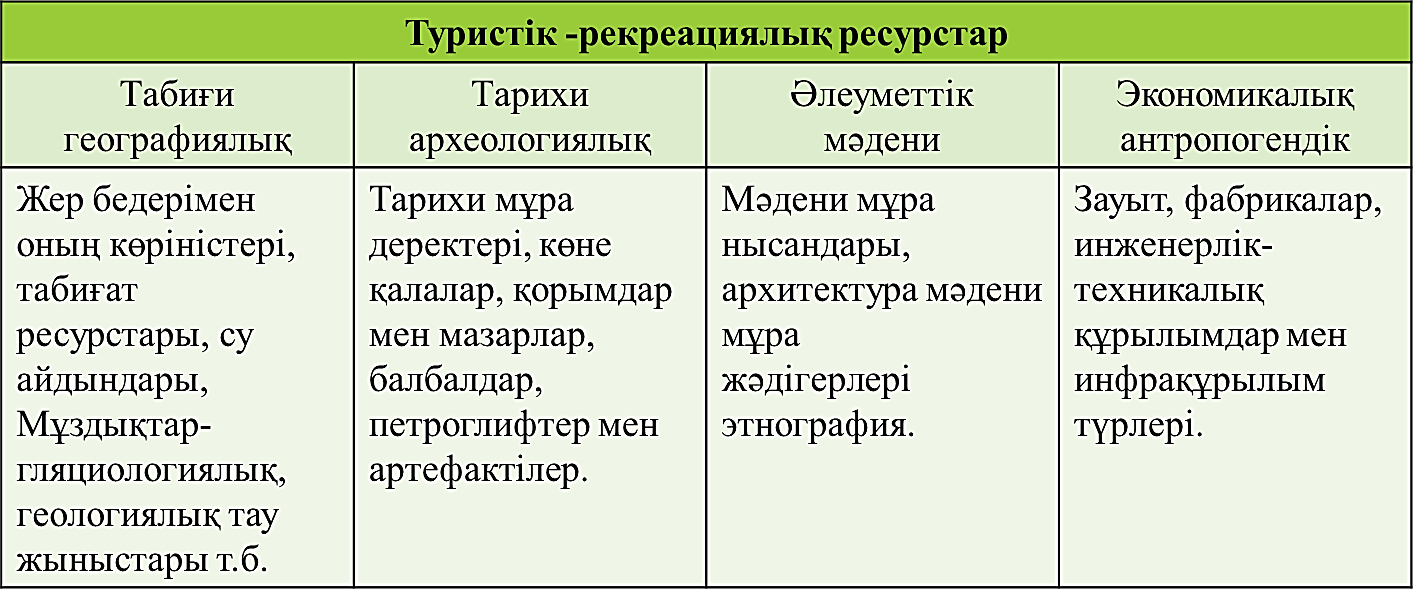
\includegraphics[width=0.8\textwidth]{assets/1110}
	\caption*{Примечание - Дерек көздері негізінде құрастырылған {[}4{]}}
\end{figure}

\begin{multicols}{2}
Жеке аумақтардың рекреациялық туристік мүмкіндіктерін бағалауда алдымен
нысандар тізілімі жасалып ресурстық әлеует анықталады. Олардың екіге
бөліп, антропогенді және табиғи ресурстар тобы деп қарастырылады.

Жеке өңірлер де туризмді дамытудың теориялық әдіснамалық астары аумақтық
рекреациялық әлеуетті бағалауға қатысты болып келеді.

Аумақтық рекреациялық әлеуетті бағалау рекреациялық ресурстарды бағалау
теориясына бағынады. Ол географиялық ресурстарды тану сферасына жатады.
Географиялық бағалауларда жеке табиғат түрлерін бағалау бағыттарында
табиғат жағдайларын бағалау жолдары қарастырылады.

Табиғат ресурстарын, табиғи орта өзгерісін, адамдардың табиғи ортада
өмір сүру деңгейін сапалы бағалауа Е.А. Котлярова, Ю.Д. Дмитриевский,
A.A. Минц, Л.И. Мухина, B.C. Преображенский, т.б. ғалымдар өз үлестерін
айтарлықтай қосты.

Қазақстандық зерттеушілер физикалық географиялық тұрғыда бағалау жолдары
арқылы жекелеген әдіснамалық мәселелер қарастырды. Олар С.Р. Ердавлетов,
В.И. Попов, Ж.Н. Алиева, О.Б. Мазбаев, Е.А. Тоқпанов, Б.К. Асубаев, М.А.
Шабельникова, М.Д. Мамадияров т.б.

Экономика ғылымдары саласы бойынша туризм мәселелері қазақстандық А.Ж.
Садуов, Г.М. Дуйсен, Р.А. Асанбаева, А.Ш. Нургалиева т.б., Г.К.Аскарова
зерттеу жұмыстарында қарастырылған {[}5{]}.

Халық шаруашылығы салалары жүйесіндегі және аумақтық еңбек бөлінісіндегі
туризмнің орны ерекше. Осыған байланысты көптеген елдерде халықтың
рекреациялық қызметтерге деген өсіп келе жатқан әлеуметтік
қажеттіліктері демалыс, рекреацияны қалыптастыруға дамытуға негіз болды.

Қазіргі географиялық және экономикалық ғылымда демалыс аймағының немесе
рекреациялық саланың шекараларын анықтау мәселесі бойынша бірыңғай
ұстаным жоқ. Зерттеу мақсаттарына байланысты әртүрлі әдіснамалық
тәсілдер қолданылуда және пікірлер қалыптасуда.

Рекреациялық, қызмет көрсету саласы бойынша оның құрамындағы туризмді
көптеген зерттеушілер бөліп көрсетеді, бұл рекреациялық тұтынудың ең тез
дамып келе жатқан тармағы.

Шаруашылық кешеніндегі туристік саладағы іс әрекеттердің орнын анықталып
отырып, ол материалдық емес өндіріс салаларына жатқызылады. Өйткені ол
туристке қажетті туристік қызметтерді қалыптастырады. Туристік сұранысты
басшылыққа алатын салалардың өнімдері қызмет көрсету түрінде әрекет
ететіндіктен, мұндай қамту аясында қарастырылатын демалыс саласы
туристік қызмет болып табылады. Жұмыс күшін қалпына келтіруді және оның
сапасын арттыруды қамтамасыз ететін туристік сала материалдық өндірістің
жұмысына тікелей әсер етеді. Рекреациялық және туристік қызметтер тек
рекреациялық нысандар, ресурстар мен инфрақұрылымды ғана емес, толықтай
әлеуметтік-экономикалық байланыстар арқылы кешенді қалыптасқан кең
әлеуметтік-экономикалық кеңістікті де қамтиды.

Туристік іс-шаралардың негізі болып туристік ресурстар саналады.
Туристік қызметтерді тікелей қалыптастырушы туристік кәсіпорындар мен
туристік инфрақұрылым, олар бірге туристік экономиканы құрайды.
Қызметтерді өндіруші ретінде ол халықтың өмір сүру деңгейін жоғарылатуда
өте маңызды рөл атқарады. Халықтың өмір сүру үшін қажетті материалдық
және мәдени-рухани нысандармен қамтамасыз етілуі, оларды тұтыну
деңгейіне жету және адамдардың осы тауарларға деген қажеттіліктерін
қанағаттандыру дәрежесі болып табылады. Туристік экономика елдің
экономикалық кешеніне қарқынды түрде еніп, туристерге қызмет көрсетумен
тығыз байланысты материалдық және материалдық емес өндірістің әртүрлі
салаларымен байланысты толықтай «туризм индустриясын» құрайды.

Қазақстан егемендік алған жылдары экономикадағы туристік саланы дамыту
туралы бірнеше құжаттар қабылдап туристік нарықты дамыту бағытында
іс-шаралар жүргізіп келеді. Туризм индустриясы немесе шаруашылық саласы
ретінде қарастыруда соңғы жылдары ғалымдар арасында әртүрлі пікірлер
қалыптасты. География ғылымның алдына аймақтағы табиғи-ресурстық
әлеуетті қолданумен байланысты мәселені қарастырудың қажеттілігіне орай
зерттеулер жүргізіле бастады. Олар аумақтық, кеңістік тұрғысында «табиғи
рекреациялық ресурс» және «рекреациялық аймақ» деген ұғымдардың
қалыптасуына ықпалын тигізді.

Экономикалық зерттеулер туристік нарық, сұраныс пен ұсыныстарға қатысты,
көпшілік жағдайда қонақүй бизнесі мен мейрамхана ісіне байланысты
жүргізілуде. Туристік-рекреациялық іс-әрекеті ұйымдастыру мәселесі
кезінде салыстырмалы түрде тауарлар мен қызметтерді тұтыну нарығының
маңызды құрамдас бөлігі, туризмді қарқынды дамытудың
ұйымдастырушылық-экономикалық тетігі бағытында қарастырылуы болатын.
Барлық салада рекреациялық тақырыптар соңғы кездерде жиі көтеріліп отыр.

Рекреациялық деген ұғым адамдардың бос уақыты кезінде демалу, сауықтыру
мақсатындағы іс әрекеттері. Қазақстандық зерттеушілер С.Р. Ердаулетов
т.б. еңбектерінде бос уақыт, демалыс, туристік әрекеттер-рекреациялық
шаралар туралы айтылады. Ғылыми әдебиеттерге шолу барысында аумақтық
туризмді дамытуға байланысты осы мәселелерге басты назар аударылды.
Территорияны пайдаланумен байланысты шаруашылық қызметтің әртүрлі
түрлері, әртүрлі шаруашылық жерлерді қажет ететіні сияқты, рекреация
үшін де әртүрлі жерлер қажет (серуендеуге, жидек өсіруге, аң аулауға,
суға түсуге, т.б.). Сонымен қатар, әрбір учаскені табиғи кешендердің
бірнеше түрін пайдаланумен байланыстыруға болады.

Бұл «аумақтық-рекреациялық жүйе» таксономиялық бірлігін енгізуге негіз
болды, сол арқылы табиғи ортаның қасиеттерін пайдалануға байланысты
рекреациялық қызметтің кез келген түрін немесе кешенін жүзеге асыруға
жарамды геожүйе деп қарастыруға болады.

Қазіргі кезде экономиканың рекреациялық бағытталған секторы үшін
экономикада «табиғи рекреациялық ресурстар» деп аталатын табиғи
ресурстардың шешуші маңызы бар, өйткені «рекреациялық қызмет» түрі мен
жалпы «туристік-рекреациялық» кешендердің мамандануы олардың саны мен
сапасына байланысты.

Ғылыми әдебиеттерде рекреациялық ресурстардың белгілі бір түрлері
егжей-тегжейлі сипатталған, олар аумақтың түріне байланысты туристік
немесе курорттық деп аталады. Дүниежүзілік туристік ұйым (ДСҰ) барлық
ресурстарды жеті үлкен топқа бөлуді ұсынды:

- табиғи ресурстар;

- энергетикалық байлық;

- демографиялық деректер мен мәдени аспектілер бойынша «адам факторы»;

- институционалдық, саяси, құқықтық және әкімшілік аспектілері;

- әлеуметтік аспектілер, әлеуметтік құрылымның ерекшеліктері, білім
беру, денсаулық сақтау және демалыс саласындағы деңгейі мен дәстүрлері;

- әртүрлі жеңілдіктер мен қызметтер, көлік, байланыс, демалыс және
ойын-сауық инфрақұрылымы;

- шаруашылық және қаржылық қызмет.

Ресурстардың бұл топтастырылуы туристік өнімді әртүрлі деңгейлерде,
соның ішінде ұлттық, аймақтық және жергілікті деңгейде қалыптастыруға
және бағалауға барынша ұтымды және кешенді көзқарасқа мүмкіндік береді.

Ерекше рөл, сөзсіз, ең алдымен аймақтың туристік-рекреациялық
мамандануын құрайтын табиғи ресурстарға тиесілі.

Табиғат ресурстары шығу тегі жағынан алғанда барлық физикалық,
биологиялық және энергетикалық ақпараттық ресурстардың жиынтығы болып
табылады, оларды пайдалану аймақтың рекреациялық сұранысы мен
мамандануына байланысты.

Сонымен экономикалық тұрғыдан алғанда, табиғи ресурстар - бұл адамдардың
қажеттіліктерін қанағаттандыру үшін өндірістік және өндірістік емес
сфераларда пайдалануға болатын табиғат элементтері мен күштері. Ал
табиғи ресурстардың әлеуметтік пайдалылығы адамның еңбек әрекеті
нәтижесінде оң немесе теріс деп өзгереді.

Соның ішінде табиғи ресурстардың өндіріс құралы ретіндегі көптеген
функцияларының ішінде оларды адамның рухани және дене күшін қалпына
келтіру құралы ретінде пайдалану өзекті бола түсуде. Көптеген табиғи
ресурстар рекреациялық және туристік әлеуетке ие, бірақ олардың көлемін
келесідей жіктеуге болады:

- шығу тегі бойынша;

- рекреациялық пайдалану түрлері бойынша;

- сарқылу жылдамдығына қарай (тез таусылатын, баяу таусылатын,
сарқылмайтын);

- мүмкін болса, өзін-өзі емдеу және өсіру (жаңартылатын, салыстырмалы
түрде жаңартылатын, қалпына келмейтін);

- мүмкіндігінше толықтыру (толтырылатын және жаңартылмайтын);

- мүмкіндігінше кейбір ресурстарды басқалармен ауыстыру (сурет 1).
\end{multicols}

\begin{figure}[H]
	\centering
	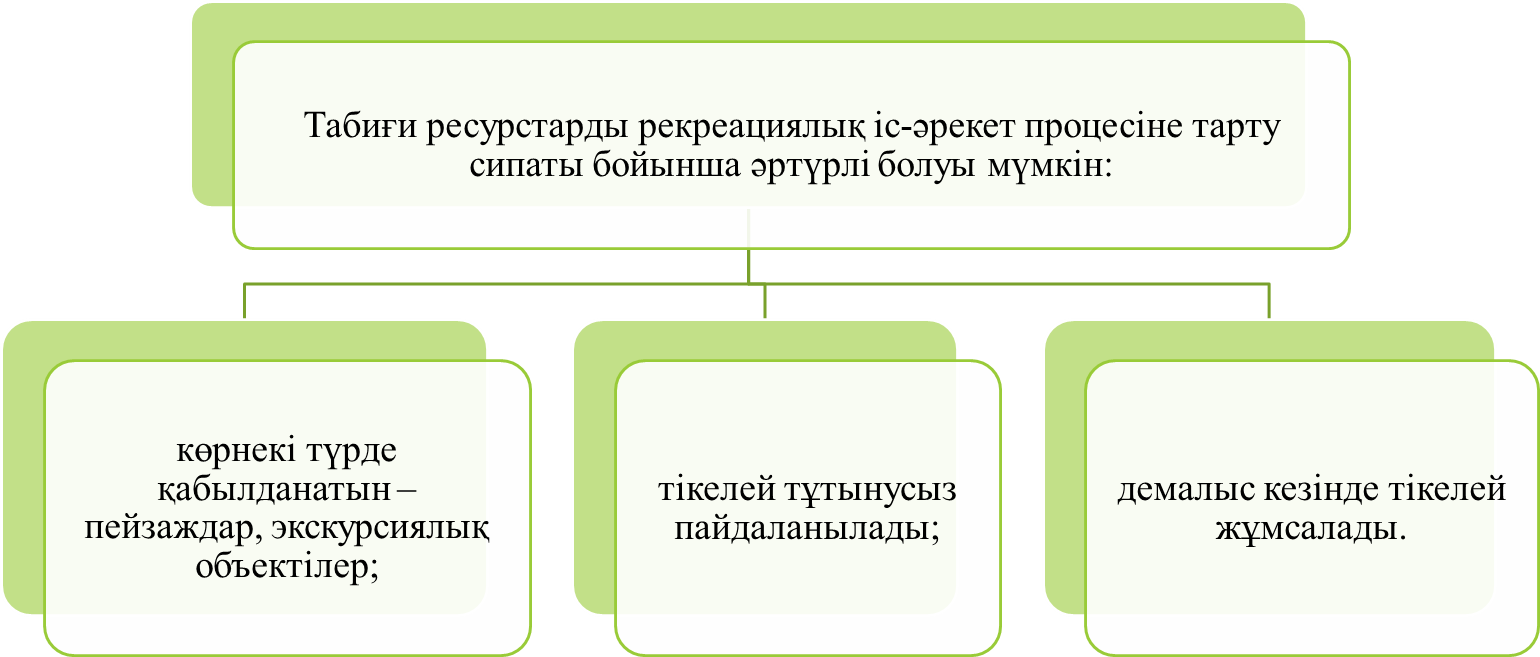
\includegraphics[width=0.8\textwidth]{assets/1111}
	\caption*{Сурет 1 -- Табиғи ресурстарды рекреациялық іс-әрекеттері {[}6{]}}
\end{figure}

\begin{multicols}{2}
Физикалық рекреациялық ресурстар - бұл физикалық-географиялық
ресурстарға (геологиялық, геоморфологиялық, климаттық, гидрологиялық
және жылулық) жіктелген жансыз табиғаттың барлық компоненттері.

Биологиялық рекреациялық ресурстар -- тірі табиғаттың барлық құрамдас
бөліктері, соның ішінде топырақ, фаунистік және флористикалық.

Энергетикалық-ақпараттық рекреациялық ресурстар - бұл аумақты немесе
ландшафтты тарту факторлары ретінде қызмет ететін және адамның
психофизикалық жағдайына жағымды әсер ететін ноосфералық сипаттағы нақты
өрістер. Ресурстың бұл түрі мәдени, сезімтал және діни туризмді
дамытудың негізі болып табылады.

Олардың әрқайсысы табиғи (қорықтар, өзен аңғарлары және т.б.),
табиғи-антропогендік (саябақтар, скверлер, орман саябақтар, ұлттық
парктер және т.б.) және бірегей ресурстар болып бөлінеді.

Бірегей күрделі рекреациялық ресурстар табиғи және табиғи-антропогендік
ландшафттардан жасанды түрде оқшауланған. Бұл рекреациялық-бағдарланған
экономиканы дамыту үшін ең тартымды туристік орындар бола отырып,
бірегей ресурстардың (табиғат ескерткіштері) ерекше маңызы бар
екендігімен түсіндіріледі.

Осы негізде табиғи рекреациялық ресурстардың түрлері анықталады:
геологиялық, геоморфологиялық, климаттық және т.б (сурет 2).
\end{multicols}

\begin{figure}[H]
	\centering
	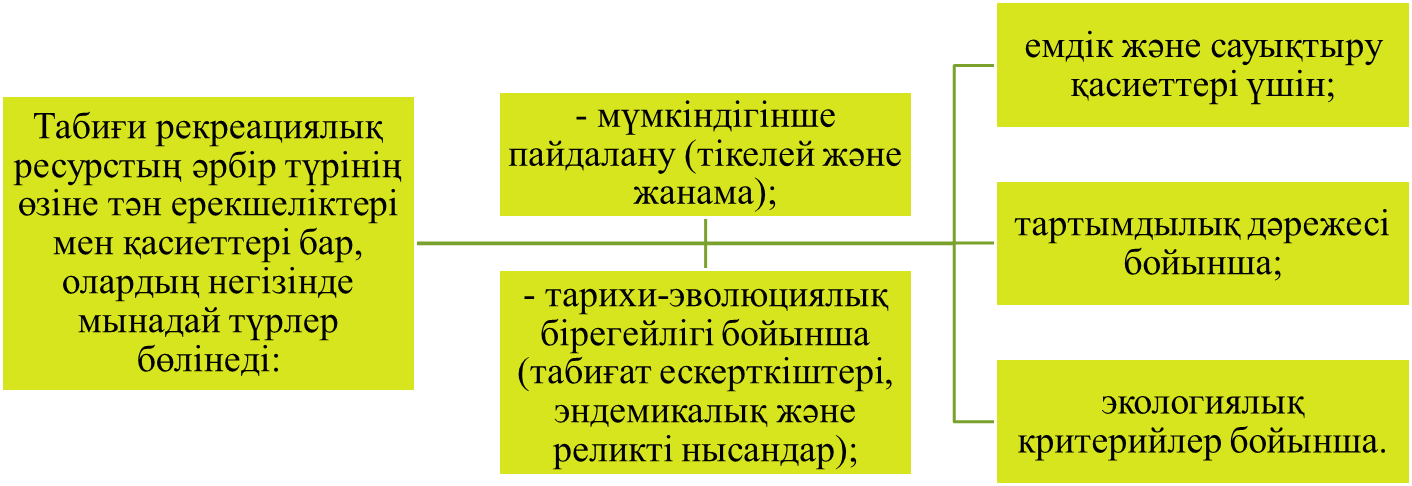
\includegraphics[width=0.8\textwidth]{assets/1112}
	\caption*{Сурет 2 -- Табиғи рекреациялық ресурстарға тән ерекшіліктері {[}7{]}}
\end{figure}

\begin{multicols}{2}
Экономикалық бағалау үшін табиғи рекреациялық ресурстарды пайдалану
мүмкіндігін анықтау қажет. Тікелей рекреациялық ресурстар деп адамның
физикалық және рухани күшін қалпына келтіруге және дамытуға тікелей
ықпал ететін табиғат күштері түсініледі. Оларға геоморфологиялық,
климаттық, гидрологиялық және энергетикалық ақпарат, флористикалық,
фаунистік және кешендік жатады. Жанама рекреациялық ресурстар тікелей
ресурстардың қалыптасуына әсер етеді. Оларға геологиялық, топырақтық,
ішінара геоморфологиялық, энергетикалық ақпарат, флористикалық және
фауналық жатады. Кешенді табиғи рекреациялық ресурстар -- адамның рухани
және дене күшін қалпына келтіру үшін медициналық, биологиялық,
эстетикалық және ғылыми құндылығы бар, бір-бірімен зат және энергия
ағындары арқылы ажырамас байланысқан барлық табиғи рекреациялық
ресурстардың жиынтығы.

Бір аймақта немесе бір аумақта жиналған табиғи рекреациялық ресурстардың
жиынтығы болған жағдайда ғана бұл аумақты рекреациялық санатқа жатқызуға
болады немесе біртұтас кешенді табиғи рекреациялық ресурс ретінде
қарастыруға болады. Рекреациялық ресурстар неғұрлым әртүрлі болса,
аймақтың рекреациялық әлеуеті және оның экономикалық даму мүмкіндіктері
соғұрлым жоғары болады.

Экономиканың туристік-рекреациялық секторының пайда болуы мен дамуының
маңызды шарты туристік және рекреациялық ресурстар мен қызметтерге
сұраныс, сондай-ақ аймақтың қолжетімділігі мен дамуы болып табылады, ол
көбінесе географиялық орналасуы мен мемлекетімен анықталады. туризм және
рекреациялық инфрақұрылым. Табиғи рекреациялық ресурстардың әрқайсысы
басқа табиғи ресурстармен үйлескенде ғана және адамның рухани және
физикалық күшін қалпына келтіру үшін пайдаланылуы мүмкін табиғи
ресурстардың кез келгені табиғи ресурстармен үйлескенде ғана тиімді
екенін атап өткен жөн. Бұл қасиетке ие болмаса, бұл әлеуетті
рекреациялық ресурс талап етілмейтін болып қалады. Демек, рекреациялық
болмайды. Мысал ретінде Солтүстік Мұзды мұхит жағалауында орналасқан
гидроминералды бұлақтарды және т.б.

Табиғи рекреациялық ресурстар міндетті пайдалану критерийі бойынша да
жіктеледі. Технологиялық міндетті немесе қажетті және технологиялық
таңдаулы немесе ілеспе табиғи рекреациялық ресурстар ажыратылады.
Бірінші топқа рекреациялық қызметтің белгілі бір түрін жүзеге асыру
мүмкін болмайтын ресурстар жатады, мысалы, қарлы тау шыңдары шаңғы
туризмі үшін қажет.

Екінші топқа рекреациялық процеске тікелей қатыспайтын, бірақ онсыз
рекреациялық процесс мүмкін емес ресурстар жатады, мысалы, таза ауыз
судың жеткілікті мөлшері, кірме жолдарды салуға қолайлы таулы жер және
т.б.

Туристік орталықтардың тұрақты дамуы үшін біртұтас рекреациялық кешенге
кіретін барлық қолда бар рекреациялық ресурстарды есепке алу мен
бағалаудың жүйелі тәсілінің маңыздылығы жоғары. Соңғысы барлық табиғи
рекреациялық ресурстар туралы мәліметтерді жинауға, олардың экономикалық
бағасын жүргізуге және болашаққа болжам жасауға мүмкіндік беретін
ақпараттық жүйелерді дамытпай мүмкін емес.

Туристік бизнесті жүзеге асыру негізгі компоненттер: капитал, заманауи
технологиялар, адам ресурстары, туристік табиғи және мәдени-тарихи
ресурстар болған жағдайда табысты жүзеге асырылуы мүмкін. Іс жүзінде
туристік аумақтарды дамыту үшін факторлар кешені қажет. Бұл қаржылық
ресурстарды тарту және заманауи технологияларды қолдану жеткіліксіз
екенін білдіреді, ең алдымен, қажетті ресурстар бар орынды таңдау немесе
оны құру керек, бұл туристік аймақтарды маркетингтің ең маңызды міндеті.
Туристік бағыттар орналастыру мүмкіндігіне қарай екі санатқа бөлінеді.
Біріншісіне туристерді көп қабылдай алатын ірі қалалар, екіншісіне
аумағы шектеулі, туристерді қабылдау мүмкіндігі шектеулі жерлер жатады.
Екінші типтегі аумақтарға теңіз жағалаулары, тау курорттары, ұлттық
саябақтар, табиғи қорықтар жатады, оларда ауданның экологиялық
тепе-теңдігін сақтау қажеттілігіне байланысты туристерді қабылдау
мүмкіндіктері шектеулі {[}8{]}.

Сонымен қатар, барлық туристік ресурстар шексіз емес, олардың белгілі
бір көлемі (потенциалды резерві), пайдалану уақыты, пайдалану
жағдайлары, құны бар екенін атап өткен жөн. Демек, туризм және
рекреациялық ресурстық ғылым арнайы зерттеу саласы ретінде туристік және
рекреациялық ресурстарды пайдалану және қорғау шарттарын анықтауды,
бағалауды және дамытуды қамтуы керек. Дегенмен, туристік аумақтардың
имиджін қалыптастыру мәселелері зерттеудің бастапқы кезеңінде ғана,
туристік аумақтардың имиджімен кәсіби негізде айналысқан отандық
мамандар іс жүзінде жоқ. Сонымен бірге туристік аймақтың ойластырылған
бейнесін жасау оның тұтынушылар алдында құндылығын арттырады, бұл өз
кезегінде нарықтық құнын арттырады. Аумақтың құнын және оның нарықтық
құнын арттыруда аумақтардың туристік-рекреациялық ресурстары ерекше рөл
атқарады.

Туристік ресурстар да шартты түрде табиғи, яғни табиғи шығу тегі және
адам әрекетінің нәтижесінде жасалған жасанды болып бөлінеді. Туризм мен
рекреацияның серпінді дамуы екі ресурстың да дамуын талап етеді, өйткені
табиғи ресурстардың өте жоғары құндылығының өзінде заманауи
инфрақұрылымның, коммуникациялардың, спорттық және демалыс орындарының
болмауы аумақтың туристік орталық ретіндегі маңыздылығына теріс әсер
етеді. Демек, толыққанды туристік аумақты қалыптастыру барлық мүдделі
тараптардың мақсатты және жүйелі іс-әрекетін талап етеді. Өз кезегінде,
туристік аумақты (орталықты) қалыптастыру бойынша ұтымды және тиімді
қызмет аумақтың туристік-рекреациялық әлеуетін бағалау саласындағы терең
зерттеулерсіз мүмкін емес, өйткені туристік аумақтардың әлеуетін болжау
туристік аумақтарды анықтауға мүмкіндік береді. Рұқсат етілетін
жүктемелер мен осы негізде аумақтардың қоршаған ортаны қорғау және
жоғалған ресурстарды молайту мақсатында шаралар әзірлеу. Мұндай
іс-шаралар туристік бизнестің табысты дамуының негізі және аумақтық
туристік өнімді өндірудің және аймақтағы инвестициялық саясаттың басым
бағыттарын жоспарлаудың бастапқы негізі болып табылады.

Облыстың ресурстық әлеуетін сауатты және тиімді басқару үшін аумақтардың
ресурстық әлеуетін бағалаудың келесі бағыттарын әзірлеу және қолдану
қажет:

- ресурстарды сандық бағалау;

- әлеуетті құрылымды, жеке потенциалды пайдалану дәрежесін бағалау;

- ресурстарды пайдалану мүмкіндіктерін бағалау.

Туристік-рекреациялық ресурстардың жай-күйін жүйелі түрде есепке алу
және олардың облыстағы туризмді дамытудағы маңызын анықтау тек
туристік-рекреациялық кадастрлар жүйесін енгізгенде ғана мүмкін болады.

Кадастр (француз тілінен аударғанда саdastre -- регистр) -- мерзімді
түрде немесе объектіге (жер, су, орман және т.б.). Туризм терминдерінің
сөздігіне сәйкес туристік ресурстар кадастры -- бұл туристік
ресурстардың жалпылама (экономикалық немесе экологиялық) тұтынушылық
(шығын немесе нүктелік) бағасы ретінде қарастырылалы.

Кадастрды құрудың негізгі мақсаты әртүрлі аймақтарда туризмді дамытудың
барлық алғышарттары мен шарттарын барынша тиімді пайдалану жолдарын
анықтау болып табылады. Ол үшін кадастр барлық туристік ресурстардың
жан-жақты сипаттамасын, оның ішінде олардың егжей-тегжейлі есепке алуын
және жіктелуін, дамудың экономикалық тиімділігін сапалық және сандық
бағалауды, пайдалануды талдауды және оның негізгі перспективаларын,
сондай-ақ туристік ресурстарды дамытудың ең маңызды шараларын қамтуы
керек. туристік және рекреациялық ресурстарды қорғау {[}9{]}.

Бұл туристік және рекреациялық ресурстардың толық сипаттамасын, олардың
тартымдылығын, көру уақытын, аумағын (көлемін), сапасын, даму немесе
пайдалану жағдайларын, уақыт бірлігінде осы ресурсты пайдалана алатын
туристер (рекреационистер) санын сандық бағалауды қамтиды. оны
сарқылтпай және экологиялық тепе-теңдікті бұзбай пайдаланудың мәні зор.
Территориялардың экономикалық дамуындағы туризм мен рекреацияның рөлін
күшейтудің заманауи жағдайында бағалау мәселелері бірінші кезектегі
мәнге ие (сурет 3).
\end{multicols}

\begin{figure}[H]
	\centering
	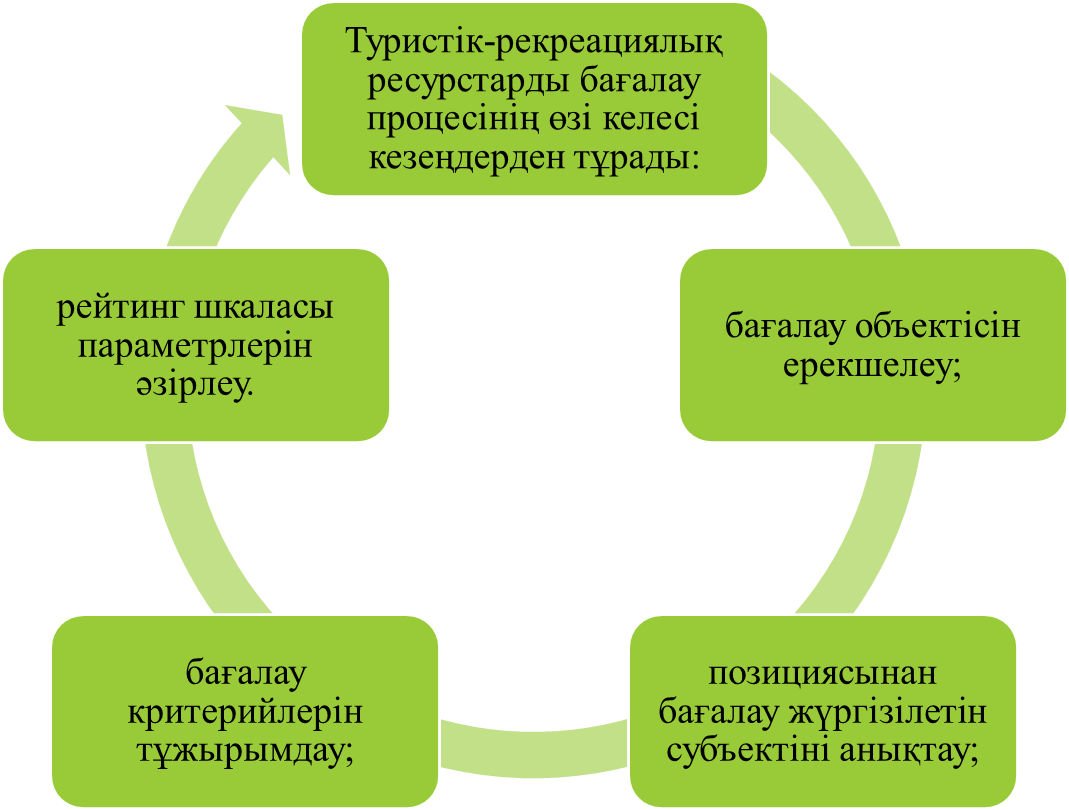
\includegraphics[width=0.6\textwidth]{assets/1113}
	\caption*{Сурет 3 -- Туристік-рекреациялық ресурстарды бағалау {[}9{]}}
\end{figure}

\begin{multicols}{2}
Шкалалар бағалау объектісі мен субъектісі арасындағы бағалау қатынасын
көрсетеді. Шкаланың 3-4 немесе 5-6 бағалау деңгейі болуы мүмкін, әрбір
деңгей берілген объектінің қасиеті мен субъектінің күйі арасындағы өзара
әрекеттесу қарқындылығының көрсеткіші болып табылады. Өзара әрекеттесу
қарқындылығы шамалыдан күштіге дейін өзгеруі мүмкін. Мәселен,
рекреацияның алғышарттарын бағалау шкаласы бес қадамнан тұрады, олардың
әрқайсысы белгілі бір градацияға сәйкес келеді:

- ең қолайлы;

- қолайлы;

- орташа қолайлы;

- аздап қолайсыз;

- қолайсыз.

Туристік және рекреациялық ресурстарды бағалаудың қолданылатын әдістері
әртүрлі, зерттеу барысында бағалаудың негізінен үш түрін қолдануға
болады: медициналық-биологиялық, психологиялық-эстетикалық және
технологиялық.

Медициналық-биологиялық бағалау табиғи факторлардың адам ағзасына әсерін
көрсетеді, мұнда климат жетекші рөл атқарады. Аумақтарды қолайлы
климаттық жағдайлар дәрежесіне қарай аудандастыруға және климаттық
терапияны кеңінен қолдануға мүмкіндік беретін, олардың адам денсаулығына
әсерін ескере отырып, климаттық факторлар кешенін бағалаудың бірқатар
әдістері әзірленді.

Психологиялық-эстетикалық бағалау табиғи ландшафт пен оның құрамдас
бөліктерінің адамға эмоционалдық әсер ету дәрежесін көрсетеді. Бұл ретте
туристік аймақта орналасқан көрікті жерлер, тарихи-мәдени және сәулет
ескерткіштері ерекше әсер етеді. Мұндай бағалау әдістері әдетте
параметрлердің әртүрлілігіне және бағалау критерийлерінің
субъективтілігіне байланысты күрделі. Дегенмен, бұл бағыттағы жұмыстар
белсенді түрде жүргізілуде, туристерді ұлттық парктердің аумақтары
бойынша бөлу зерттелуде. Бұл зерттеулердің нәтижелері шеткі аймақтардың
(екі орта арасындағы шекаралық жолақтар: су-жер (күшті әсер),
орманды-сала (орташа әсер), төбе-жазық (әлсіз әсер) ең жоғары және ең
тартымды әсер ететінін көрсетті.

{\bfseries Нәтижелер мен талқылау.} Аумақтарға географиялық-туристік талдау
жасауда рекреациялық әлеуетке жататындар:

- физикалық географиялық сипаттама бере отырып, табиғат ортасының
қолайлылығын, мүмкіндігін анықтау;

- ландшафтық жер жағдайын рекреациялық бағалай, олардың
аттрактивтілігін, экологиялық жай-күйін анықтау;

- аумақтық жергілікті тұрғыда туристік ресурстар реестрін құрастыру,
оның туристік жағдайын саралау;

- туристік-рекреациялық нысандарды пайдалану дәрежесін анықтап,
рекреациялық мүмкіндіктеріне шолу беру;

- туристік пайдалануына сай оларды аудандастыру.

Психологиялық-эстетикалық бағалаудың басқа әдістерімен қатар соңғы
уақытта экзотикалық және бірегейлік дәрежесі зерттелді. Экзотикалық
демалыс орнының тұрақты тұрғылықты жеріне қатысты қарама-қарсылық
дәрежесі ретінде, ал бірегейлік - заттардың немесе құбылыстардың
бірегейлік дәрежесі ретінде анықталады.

Технологиялық бағалау белгілі бір туризм немесе рекреация түріне
аумақтың жарамдылығын, сондай-ақ оның инженерлік және құрылыстық даму
мүмкіндігін бағалауға мүмкіндік береді.

Бағалау жұмысының қорытынды кезеңі -- интегралды бағалаудың қорытындысы
және бағалау формасын таңдау. Әдетте екі ауыспалы форма қолданылады:
сапа және нүкте. Сапалық бағалаудың күштілігі ол бағалау ерекшеліктерін
логикалық негіздеуге мүмкіндік береді. Бұл тәсіл нүктелік бағалауды
жақсырақ негіздеуге ықпал етеді, оның айрықша белгілері өрнектің
қысқалығы, анықтығы және салыстыру мүмкіндігі болып табылады.

{\bfseries Қорытынды.} Жоғарыда айтылғандарды талдай отырып, табиғи
рекреациялық ресурстар туристік өнімді қалыптастыруда орталық маңызы бар
деп айтуға болады. Алайда энергетика, көлік, байланыс, еңбек ресурстары
сияқты ресурстар көбінесе аумақ пен аймақтың рекреациялық әлеуетін
құрайды, өйткені олар мерекені жайлы, мәдениетті және қызықты өткізу.
Туристік-рекреациялық әлеуеттің негізгі қағидаттары мынадай болып
келеді. Мәселен, рекреациялық әрекеттерде оның алуан-түрлілігі туризм
жіктеліміне сәйкестігі мен оның демалу рекреациялық мүмкіндіктерін
жатқызуға болатындар:

- туристік ресурстардың өзіндік ерекшелігі, бірегейлігі;

- адамдардың қоршаған ортаға деген экологиялық көзқарасы;

- пайдаланатын ресурстардың мөлшері мен көлемі.

Рекреациялық бағалаудың жолдары әртүрлі болып келеді. Өңірдің ресурстық
әлеуетін сауатты және тиімді басқару үшін ресурстардың сандық бағасын
әзірлеу және қолдану, әлеует құрылымы мен жеке әлеуетті пайдалану
дәрежесін бағалау, пайдалану мүмкіндіктеріне нақты баға беру қажет.
Туристік ресурстардың шексіз емес екенін түсіну керек, олардың белгілі
бір потенциалдық қоры, оларды пайдалану уақыты, пайдалану шарттары мен
құны бар.

Нәтижесінде туризм және рекреациялық ресурстық ғылым туристік және
рекреациялық ресурстарды пайдалану және қорғау шарттарын анықтауды,
бағалауды және дамытуды қамтуы керек. Қазіргі уақытта туристік
аумақтардың имиджін қалыптастыруға қатысты мәселелер тек зерттеудің
бастапқы сатысында тұр және кәсіби негізде туристік аумақтардың
имиджімен айналысқан отандық мамандарды жетілдіру орынды. Сонымен бірге
туристік аймақтың ойластырылған бейнесін жасау оның тұтынушылар алдында
құндылығын арттырады, бұл өз кезегінде нарықтық құнын арттырады.
Аумақтың құнын және оның нарықтық құнын арттыруда аумақтардың
туристік-рекреациялық ресурстары ерекше рөл атқарады.
\end{multicols}

\begin{center}
{\bfseries Әдебиеттер}
\end{center}

\begin{noparindent}
1. Ердавлетов С.Р., Искакова К.А., Артемьев А.М., Баяндинова С.М.
Рекреационный туризм: учеб. пособие. -- Алматы: Қазақ университеті,
2017. -- 214 с.

2. Зырянов А.И. Теория и методология рекреационной географии: учебное
пособие. - Пермь: Пермский государственный национальный
исследовательский университет, 2021. - 368 с.

3. Назаркина В.А., Владыкина Ю.О., Воротникова Е.Ю. Виды и тенденции
развития туризма: учебное пособие. -Новосибирск: Новосибирский
государственный технический университет, 2014. - 235 с.
ISBN978-5-7782-2437-7

4. Плохих Р.В., Исаков Е.Д., Актымбаева А.С. Туризмология негіздері: оқу
құралы. -- Алматы: Қазақ Университеті, 2021. -- 112 б.

5. Абишева З. М. Основы туристско-краеведческой работы: учебное пособие.
-- Алматы, «Қазақ университеті», 2018. -- 106 с.

6. Уварова А.К., Сабиров Д.З. Туристік-рекреациялық картографиялау курсы
бойынша лабораториялық және тәжірибелік жұмыстарды орындау нұсқаулығы.
-- Алматы: Қазақ университеті, 2016. -- 138 б.

7. Абишева З.М., Абдреева Ш.Т. Туристік өлкетану жұмыстарының негіздері:
оқу құралы. -- Өңд. толықт. 2-бас. -- Алматы: Қазақ университеті, 2019.
-- 122 б.

8. Артемьев А.М. Абдреева Ш.Т., Актымбаева А.С. Методические
рекомендации по определению норм рекреационных нагрузок на туристские
маршруты и экологические тропы особо охраняемых природных территорий
ПРООН. - Нур-Султан, 2020 г. -- 78 с

9. Шәкен А.Ш. Ердавлетов С.Р. Туризм Казахстана: учебное пособие. -
Алматы, Бастау 2015. -- 520 с
\end{noparindent}

\begin{center}
{\bfseries References}
\end{center}

\begin{noparindent}
1. Erdavletov S.R., Iskakova K.A., Artem\textquotesingle ev A.M.,
Bayandinova S.M. Rekreatsionnyi turizm: ucheb. posobie. -- Almaty: Kazak
universitetі, 2017. - 214 s {[}in Kazakh.{]}

2. Zyryanov A.I. Teoriya i metodologiya rekreatsionnoi geografii:
uchebnoe posobie. - Perm\textquotesingle: Permskii

gosudarstvennyi
natsional\textquotesingle nyi issledovatel\textquotesingle skii
universitet, 2021. - 368 s. {[}in Russian{]}

3. Nazarkina V.A., Vladykina Yu.O., Vorotnikova E.Yu. Vidy i tendentsii
razvitiya turizma: uchebnoe posobie. -Novosibirsk: Novosibirskii
gosudarstvennyi tekhnicheskii universitet, 2014. - 235 s.
ISBN978-5-7782-2437-7 {[}in Russian{]}

4. Plokhikh R.V., Isakov E.D., Aktymbaeva A.S. Turizmologiya negіzderі:
oku kuraly. -- Almaty: Kazak Universitetі, 2021. -- 112 b. {[}in
Kazakh.{]}

5. Abisheva Z. M. Osnovy turistsko-kraevedcheskoi raboty: uchebnoe
posobie. -- Almaty, «Kazak universitetі», 2018. -- 106 s. {[}in
Russian{]}

6. Uvarova A.K., Sabirov D.Z. Turistіk-rekreatsiyalyk kartografiyalau
kursy boiynsha laboratoriyalyk zhane tazhіribelіk zhumystardy oryndau
nuskaulygy. -- Almaty: Kazak universitetі, 2016. -- 138 b. {[}in
Kazakh.{]}

7. Abisheva Z.M., Abdreeva Sh.T. Turistіk өlketanu zhumystarynyn
negіzderі: oku kuraly. -- Ond. tolykt. 2-bas. -- Almaty: Kazak
universitetі, 2019. -- 122 b. {[}in Kazakh{]}

8. Artem\textquotesingle ev A.M. Abdreeva Sh.T., Aktymbaeva A.S.
Metodicheskie rekomendatsii po opredeleniyu norm

rekreatsionnykh
nagruzok na turistskie marshruty i ekologicheskie tropy osobo
okhranyaemykh prirodnykh territorii PROON. - Nur-Sultan, 2020 g. -78 s.
{[}in Russian{]}

9. Shәken A.Sh. Erdavletov S.R. Turizm Kazakhstana: uchebnoe posobie. -
Almaty, Bastau 2015. -- 520 s. {[}in Russian{]}
\end{noparindent}

\emph{{\bfseries Авторлар туралы мәліметтер}}

\begin{noparindent}
Д.И. Джангельдина -- п.ғ.к., доцент, Қазақ технология және бизнес
университеті, Астана, Қазақстан, e-mail: dariga\_da@mail.ru;

С.М. Рустемова -- магистр, аға оқытушы, Қазақ технология және бизнес
университеті, Астана, Қазақстан, e-mail: sabiruwa1986@mail.ru;

Е.Б. Абеуханова -- магистр, аға оқытушы, Қазақ технология және бизнес
университеті, Астана, Қазақстан, e-mail: erkejana77@mail.ru;

К.А. Омарова -- магистр, аға оқытушы, Қазақ технология және бизнес
университеті, Астана, Қазақстан, e-mail: omarova820204@mail.ru;

Г.Б. Ахметова -- магистр, аға оқытушы, Қазақ технология және бизнес
университеті, Астана, Қазақстан, e-mail: galiya\_hanum @mail.ru.
\end{noparindent}

\emph{{\bfseries Information about the authors}}

\begin{noparindent}
D.I. Dzhangeldina -- Ph.D., Associate Professor, Kazakh University of
Technology and Business, Astana, Kazakhstan, e-mail: dariga\_da@mail.ru;

CM. Rustemova -- Master's degree, senior lecturer, Kazakh University of
Technology and Business, Astana, Kazakhstan, e-mail:
sabiruwa1986@mail.ru;

E.B. Abeukhanova -- Master's degree, senior lecturer, Kazakh University
of Technology and Business, Astana, Kazakhstan, e-mail:
erkejana77@mail.ru;

K.A. Omarova -- Master's degree, senior lecturer, Kazakh University of
Technology and Business, Astana, Kazakhstan, e-mail:
omarova820204@mail.ru;

G.B. Akhmetova -- Master's degree, senior lecturer, Kazakh University of
Technology and Business, Astana, Kazakhstan, e-mail: galiya\_hanum
@mail.ru.
\end{noparindent}
